\documentclass[10pt,a4paper,twocolumn]{article}

% Packages (alphabetical order)
\usepackage{amsmath,amssymb}
\usepackage{balance}
\usepackage{booktabs}
\usepackage{caption}
\usepackage[margin=17mm]{geometry}
\usepackage{graphicx}
	\graphicspath{
		{./}
		{../graphics/}
	}
\usepackage{hyperref}
\hypersetup{
  	bookmarks=true,
    unicode=false,
    pdftoolbar=true,
    pdfmenubar=true,
    pdffitwindow=true,
    pdftitle={Multi-agent systems},
    pdfauthor={},
    pdfsubject={},
    pdfnewwindow=true,
    pdfkeywords={},
    colorlinks=true,
    linkcolor=blue,
    citecolor=blue,
    filecolor=blue,
    urlcolor=blue
}
\usepackage{lipsum}
\usepackage{microtype}
\usepackage[numbers,sort&compress]{natbib}
	\bibliographystyle{apalike2}

% Title information
\title{Stigmergic Coordination in UAV Search and Rescue:\\A Behavioral Sensitivity Analysis}
\author{
  Arthur Schauwvlieghe \\
  {\small KU Leuven} \\
  \texttt{arthur.schauwvlieghe@student.kuleuven.be}
  \and
  Guust Delbaere \\
  {\small KU Leuven} \\
  \texttt{guust.delbaere@student.kuleuven.com}
  \and
  Harun Kalkanci \\
  {\small KU Leuven} \\
  \texttt{harun.kalkanci@student.kuleuven.be}
}
\date{}

\begin{document}
\maketitle

\begin{abstract}
Efficient search and rescue in large, unknown environments remains a fundamental challenge for autonomous systems. We present a multi-agent model of Unmanned Aerial Vehicle (UAV) search and rescue that combines Belief-Desire-Intention (BDI) statechart reasoning with a reversed Ant Colony Optimization (ACO) mechanism. Standard ACO models use pheromones to attract agents to rewarding locations. In our model, agents treat pheromone as a collective spatial memory of recently covered ground and are repelled by it. This mechanism ensures the fleet spreads out to avoid redundant search efforts. When a UAV detects a victim, it follows an attractive signal directly toward the target. This dual-signal approach creates a dynamic Explore-Exploit balance without the need for centralized scheduling. 

Every agent transition is made explicit and auditable through the use of hierarchical BDI state charts. Our work provides a full AnyLogic implementation that integrates these logical structures with essential modules such as victim placement, pheromone grids, and battery management logic. An automated experimental pipeline then evaluates the system through large-scale parameter sweeps. These results characterize how ACO scoring exponents, step length, and candidate count jointly shape the convergence speed and reliability of the swarm.
\end{abstract}

% ─────────────────────────────────────────────────────────────────────────────
\section{Introduction}
% ─────────────────────────────────────────────────────────────────────────────

Search and rescue operations are extremely time-critical because the probability of survival decreases rapidly as time passes. Ground teams are often constrained by difficult terrain and face the same hazards as the victims they seek. Unmanned Aerial Vehicles (UAVs) offer a superior alternative as they can be airborne in minutes and traverse large areas at high speeds regardless of the ground conditions.

The central challenge for any multi-UAV mission is effective coordination. Traditional solutions often rely on a central station to partition the search space and assign tasks. However, this architecture is fragile in disaster zones where communication is unreliable and the central controller represents a single point of failure. Decentralized multi-agent systems offer a more resilient approach by using local rules and shared environmental cues. This method is inspired by social insects and remains robust even if individual agents fail as it does not require a global view \citep{bk:Bonabeau1999}.

This paper presents a compact model of decentralized UAV search and rescue implemented in AnyLogic. Our model uses two main design principles. First, UAVs coordinate through a reversed Ant Colony Optimization (ACO) mechanism where pheromones mark covered ground to repel future agents. This guides the swarm toward unexplored territory. Second, agent logic is defined by a statechart inspired by the Belief-Desire-Intention (BDI) architecture \citep{bk:Wooldridge2009}. This makes behavioral modes and transition conditions explicit and easy to analyze.

Our contributions include a complete agent-based model with three interacting agent types. We formalize the scoring function for reversed ACO and explain how it governs the balance between exploration and exploitation. Finally, we establish an automated experimental pipeline to characterize how movement rules and behavioral parameters shape global search performance.

% ─────────────────────────────────────────────────────────────────────────────
\section{Background}
% ─────────────────────────────────────────────────────────────────────────────

\paragraph{Agent-Based Modelling and Multi-Agent Systems}
ABM is a powerful tool for studying complex systems by simulating the behaviours of autonomous individuals \citep{ar:Schelling1971,ar:Macal2016}. This approach allows macro-level phenomena to emerge from simple micro-level rules. A classic example is Reynolds' boids model, where agents follow basic steering rules, such as separation and alignment, to produce coherent flocking patterns \citep{inpr:Reynolds1987}. In the context of SAR, this framework provides a way to analyse how individual agent-level choices translate into collective search efficiency.

\paragraph{Belief-Desire-Intention Architecture}
The BDI architecture is a common framework for designing rational agents \citep{bk:Bratman1987,inpr:RaoGeorgeff1991}. In this model, beliefs represent the information an agent has about its environment. Desires are the long-term objectives the agent wants to achieve. Intentions are the specific plans the agent commits to executing in order to fulfil its desires based on its current beliefs. This architecture allows agents to balance goal-oriented behaviour with the flexibility to react to new information from their sensors.

\paragraph{Ant Colony Optimization and Stigmergy}
Coordination in MAS is often achieved through stigmergy, where agents communicate indirectly by modifying their shared environment \citep{bk:Bonabeau1999}. ACO is a well-known metaheuristic inspired by this principle \citep{ar:Dorigo1996,bk:Dorigo2004}. In natural ant colonies, individuals deposit pheromones on the ground to mark successful paths to food sources. Future agents are attracted to these markers, which creates a positive feedback loop that leads the group toward efficient solutions. This coordination mechanism requires no direct communication between agents and is highly effective for solving complex spatial search problems.

% ─────────────── full-width statechart figure ─────────────────────────────
\begin{figure*}[ht]
    \centering
    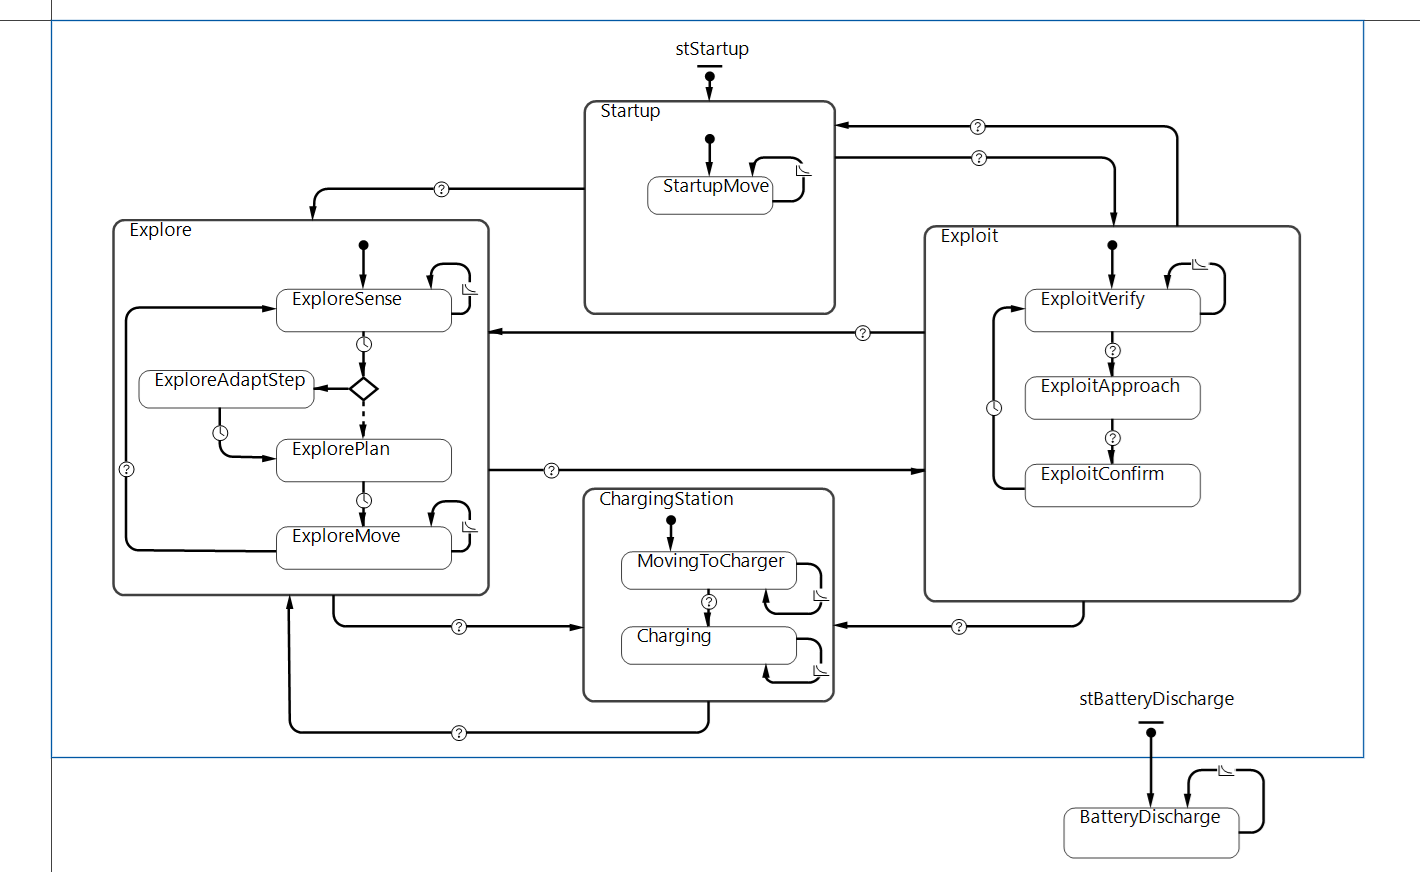
\includegraphics[width=\textwidth]{img/statechart.png}
    \caption{The BDI-inspired UAV statechart shows the primary behavioral modes. The \texttt{Startup} mode manages the movement to initial dispersal points. The \texttt{Explore} mode uses pheromone logic to search the environment. The \texttt{Exploit} mode handles victim confirmation and approach. The \texttt{ChargingStation} mode handles battery replenishment at the base. Finally, the \texttt{BatteryDischarge} state runs in parallel to simulate continuous energy consumption.}
    \label{fig:statechart}
\end{figure*}

% ─────────────────────────────────────────────────────────────────────────────
\section{Design}
% ─────────────────────────────────────────────────────────────────────────────

A set of foundational design choices guides our approach to decentralized coordination. These high-level principles govern how the fleet explores the search area and responds to discovered victims.

\paragraph{Pheromone Repulsion}
The core of our coordination system is the use of repulsive pheromones. While standard ACO \citep{ar:Dorigo1996} uses pheromones as an attractor, we invert this signal to suit a SAR mission. In our model, high pheromone levels indicate that a UAV has recently passed over a specific grid cell. By scoring candidate waypoints inversely to their pheromone intensity, we ensure that the swarm avoids redundant coverage and is naturally pushed toward unexplored territory. These pheromones evaporate over time to represent a decaying spatial memory. This allows agents to eventually return to older areas, accounting for the possibility that a victim was missed or that environmental conditions have changed.

\paragraph{Exploration--Exploitation Duality}
The repulsive pheromone signal is balanced by an attractive signal from victim detections. This interaction creates a dynamic balance between exploration and exploitation that adapts to the mission state. In the absence of detections, pheromone repulsion dominates and forces agents to spread out into unsearched space. When a UAV identifies a victim, this exploratory behaviour is immediately overridden by a direct approach to the target. Following a successful confirmation, the agent remains in the vicinity briefly to perform a local search. This strategy allows the swarm to capitalize on the spatial structure of the environment by focusing resources where they are most likely to find more victims.

\paragraph{Victim Placement Model}
\label{sec:design_victim}
We model victim placement using a Gaussian Mixture Model (GMM) to simulate the realistic spatial clustering found in disaster sites. Structural collapses or flooding events rarely result in victims being spread uniformly across a search area. Instead, victims tend to be concentrated in high-impact zones. Using a GMM allows us to generate these clusters and test the effectiveness of our local search bias. By varying the number and spread of these clusters, we can evaluate the robustness of our coordination strategy across a range of disaster scenarios, from single-point incidents to widely dispersed multi-site emergencies.

% ─────────────────────────────────────────────────────────────────────────────
\section{System Model}
% ─────────────────────────────────────────────────────────────────────────────

This section describes the mathematical and logical structure of the simulation. We define the environment and the behaviors of each agent type to provide a clear view of the swarm dynamics.

\paragraph{The Environment}
The simulation takes place in a continuous area of $45 \times 25$ meters, as shown in Figure~\ref{fig:simulation}. We overlay this space with a shared pheromone grid to coordinate the swarm. Colored squares on the map indicate recently visited locations, where the intensity of the coverage can be read from the legend on the right. This space is inhabited by two UAV agents and five Victim agents. The Victim agents act as passive data containers that store their specific location and discovery status. They contain no internal logic and remain stationary throughout the mission for the sake of simplicity. The Main agent then orchestrates the simulation by initializing the environment and placing targets according to a GMM. This orchestrator also manages the pheromone grid and applies a lazy exponential decay model to simulate evaporation over time:
\begin{equation}
    \tau(t) = \tau_0 \cdot e^{-\rho (t - t_0)} .
\end{equation}
In this model, $\tau(t)$ represents the current pheromone level, and $\tau_0$ is the level recorded at the last update time $t_0$. The parameter $\rho$ sets the evaporation rate. This decay ensures that the spatial memory of the swarm remains dynamic and responsive to recent sensor data.

% ─────────────── Full-width simulation figure ─────────────────────────────
\begin{figure*}[ht]
    \centering
    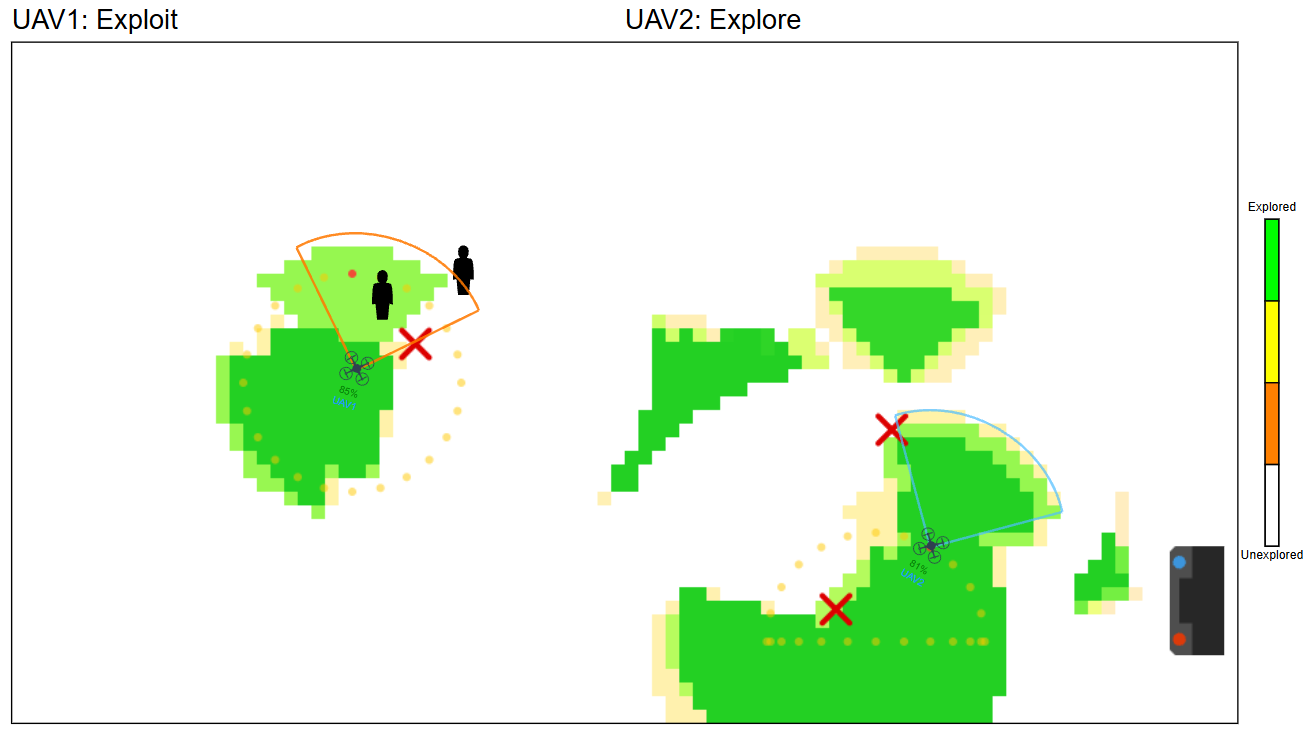
\includegraphics[width=\textwidth]{img/simulation.png}
    \caption{Snapshot of the running simulation showing the pheromone distribution, where green tones indicate high coverage and white indicates unexplored territory. UAV2 on the right is in \texttt{Explore} mode, with its blue sensor cone sweeping the area ahead. UAV1 on the left is in \texttt{Exploit} mode, with an orange cone indicating an active victim detection. Red crosses mark victims that have already been confirmed.}
    \label{fig:simulation}
\end{figure*}

\paragraph{Agent Behaviour}
Once the environment is set up, we define how the agents behave within it. Each UAV follows a BDI architecture implemented through the hierarchical state chart shown in Figure~\ref{fig:statechart}. At the start of the mission, agents enter a \texttt{Startup} phase to reach pre-assigned dispersal positions. This ensures that the fleet begins the search with minimal overlap. Once in position, each UAV enters the main behavioural cycle, where it switches between the \texttt{Explore} and \texttt{Exploit} parent states. An orthogonal state called \texttt{BatteryDischarge} runs in parallel throughout the flight to simulate the continuous depletion of the battery at a constant rate.

\paragraph{Searching for Victims}
The core of this behavioural cycle is the search process within the \texttt{Explore} parent state. This mode implements a reversed ACO logic to cover the area. As shown in Figure~\ref{fig:simulation}, each UAV considers a ring of $n$ yellow candidate waypoints. The radius of this ring is called the step length $d$. The agent scores each candidate $i$ based on the local pheromone level $\tau_i$ and the staleness $\eta_i$ of the grid cell:
\begin{equation}
    s_i = \left(\frac{1}{1 + \tau_i}\right)^{\alpha} \cdot \eta_i^{\beta} .
\end{equation}
In this scoring function, $\alpha$ and $\beta$ are exponents that weight the importance of pheromone repulsion and staleness attraction. Staleness is derived from the freshness $f_i$ of a cell, which tracks the time since it was last sensed:
\begin{equation}
    f_i(t) = \max\left(0,\; 1 - \frac{t - t_{\mathrm{last},i}}{T_{\mathrm{stale}}}\right) .
\end{equation}
The term $t_{\mathrm{last},i}$ is the timestamp of the last visit, and $T_{\mathrm{stale}}$ is a constant that defines when a cell is considered completely stale. Within the \texttt{ExploreSense} and \texttt{ExplorePlan} sub-states, the agent evaluates these scores and chooses a destination marked by a red circle in the simulation. The UAV then transitions to \texttt{ExploreMove} to fly toward the target.

If the local area is already heavily covered, an \texttt{ExploreAdaptStep} node allows the UAV to escape the saturated neighbourhood. This mechanism checks the minimum pheromone level $\tau_{\min}$ among all candidates on the ring. When $\tau_{\min}$ is high, it indicates that even the least-explored candidate is in a well-covered region. In this case, the UAV increases its step length to jump further into fresh territory:
\begin{equation}
    d_{\mathrm{current}} = d \cdot \min\left(M,\; 1 + \tau_{\min}\right) .
\end{equation}
The parameter $M$ acts as a maximum multiplier to keep the jump distance within a reasonable range. This adaptive behaviour prevents the UAV from wasting time in areas that have already been thoroughly searched.

\vspace{1cm}
\paragraph{Confirming detections}
A detection within the sensor cone initiates a transition to the \texttt{Exploit} parent state. As shown in Figure \ref{fig:simulation}, this shift is visible when the sensor cone of a UAV changes from blue to orange. The agent first enters the \texttt{ExploitVerify} sub-state to confirm the signal through a secondary sensing sweep before navigating to the target. Once the UAV reaches the victim, the \texttt{ExploitConfirm} state handles the final logging and mission statistics. This discovery is marked with a red cross on the map and the Main agent clears the nearby pheromone grid. The white unexplored zone surrounding the victim in the bottom right of Figure \ref{fig:simulation} illustrates this reset which encourages the swarm to re-examine the area. After the confirmation is complete, the agent returns to the \texttt{Explore} mode.

\paragraph{Battery and Charging}
When the battery level drops below a set threshold, the agent preempts its current task and enters the \texttt{ChargingStation} parent state. During the \texttt{MovingToCharger} phase, the UAV suspends non-essential operations like sensing and pheromone deposition. This energy saving mode halves the battery depletion rate while the agent travels toward the charging station at the bottom right of the environment. After reaching this location, the UAV enters the \texttt{Charging} sub-state to replenish its power. Once the battery is fully recharged, the agent uses its saved coordinates to return to the search area and resume its mission.

% ─────────────────────────────────────────────────────────────────────────────
\section{Experimental Setup}
% ─────────────────────────────────────────────────────────────────────────────

To characterize how search performance responds to the model's key behavioral parameters, we run two complementary experiments using AnyLogic's built-in sweep infrastructure, with sensor range fixed at 5\,m. The first sweeps all four parameters in a full factorial grid to expose their joint interactions. The second holds three parameters at their defaults and varies only one at a time, isolating the individual effect of each parameter in turn.

\textbf{Candidate count} ($n$) controls the angular resolution of the waypoint selection ring: more candidates offer a finer-grained directional choice and a smoother score distribution, at the cost of additional scoring operations per planning step. We vary $n \in \{12, 18, 24, 30, 36\}$.

\textbf{Step length} ($d$) sets the radius of the candidate circle in meters, determining how far the UAV moves at each planning step. Longer steps increase the rate of area coverage but reduce spatial resolution and the ability to target specific nearby cells precisely. We vary $d \in \{2.5, 3.75, 5.0, 6.25, 7.5\}$\,m.

\textbf{Pheromone exponent} ($\alpha$) controls the weight of the pheromone repulsion term in Equation~\eqref{eq:aco}. A higher value makes the scoring function more sensitive to pheromone differences, producing stronger and more decisive avoidance of recently covered cells. We vary $\alpha \in \{0.5, 1.0, 1.5, 2.0, 2.5\}$.

\textbf{Staleness exponent} ($\beta$) controls the weight of the cell-age term. A higher value gives stronger preference to cells that have not been sensed recently. We vary $\beta \in \{1.0, 1.5, 2.0, 2.5, 3.0, 3.5, 4.0\}$. In practice, because our pheromone evaporation rate is kept very low and victims do not move, recently explored cells never become genuinely stale and $\beta$ has limited impact on outcomes.

We evaluate each parameter combination across 10 independent random seeds. The seed determines both the victim placement (GMM sampling) and the stochastic choices in waypoint selection. Replicating across seeds ensures that observed performance differences reflect genuine parameter sensitivity rather than idiosyncrasies of a particular victim configuration.

We record two primary metrics per run. \textbf{Convergence time} is the simulation time at which the last victim is confirmed found. \textbf{Convergence rate} is the fraction of runs for a given parameter configuration in which all victims are found before the 200-second safety-stop limit. Runs that time out are recorded with an undefined convergence time and reduce the convergence rate of their configuration. The dual-metric approach distinguishes configurations that are consistently fast from those that succeed on only some seeds, an important distinction for evaluating robustness.

The experimental pipeline is fully automated. Each run writes its result incrementally to a CSV log file in a numbered experiment folder, allowing runs to proceed in parallel without coordination beyond synchronized file writes. When all runs complete, a Python post-processing script picks up the CSV files automatically and produces the full set of visualizations without manual intervention. A snapshot of the running simulation, illustrating the pheromone grid, UAV sensor cones, and victim locations, is shown in Figure~\ref{fig:simulation}.

% ─────────────────────────────────────────────────────────────────────────────
\section{Results and Discussion}
% ─────────────────────────────────────────────────────────────────────────────

One implementation choice shapes all the results because in our simulation, victims are stationary and do not change location after placement. Because the underlying search objective does not change, we set the pheromone evaporation rate to a very low value. Pheromone deposited on a cell effectively persists for the duration of a run, making recently explored territory reliably repulsive. This also explains why the staleness exponent $\beta$ has little measurable effect because cells never genuinely become stale when the state of the world does not change beneath them.

\subsection{Step Length Sweep}

The step length sweep isolates the effect of the planning ring radius on search performance.
Twenty independent random seeds (1--20) are evaluated across eight fixed step lengths
$d \in \{1.25, 2.5, 3.75, 5.0, 6.25, 7.5, 8.75, 10.0\}$\,m.
All other parameters are held at their defaults: $n = 24$ candidate waypoints,
$\alpha = 1.0$, $\beta = 1.0$, and a sensor range of 5\,m.
The adaptive step mechanism is disabled for all fixed-step conditions, ensuring that the
configured ring radius is the one actually used throughout each run.
A ninth condition, the ``Default (adaptive)'' baseline, re-runs the same 20 seeds with
adaptive scaling enabled and a base step of $d = 4$\,m, providing a direct comparison
between fixed and adaptive strategies under otherwise identical settings.

Steps of 2.5 and 5.0\,m achieve the highest convergence rate at 76\,\%, making them jointly
optimal within the evaluated range.
The shortest step ($d = 1.25$\,m) achieves the fastest mean convergence time among runs that
do converge (44.7\,s $\pm$ 14.6\,s SD), but its convergence rate is only 26\,\%,
meaning most runs fail to locate all victims within the time limit.
Steps in the mid-range (3.75--7.5\,m) plateau at 60--76\,\%, with mean convergence times
between 53 and 70\,s and substantial run-to-run variance.
The default adaptive configuration converges on only 45\,\% of seeds with a mean time
of 55.8\,s, underperforming most fixed-step alternatives on both metrics.

\begin{figure}[h]
    \centering
    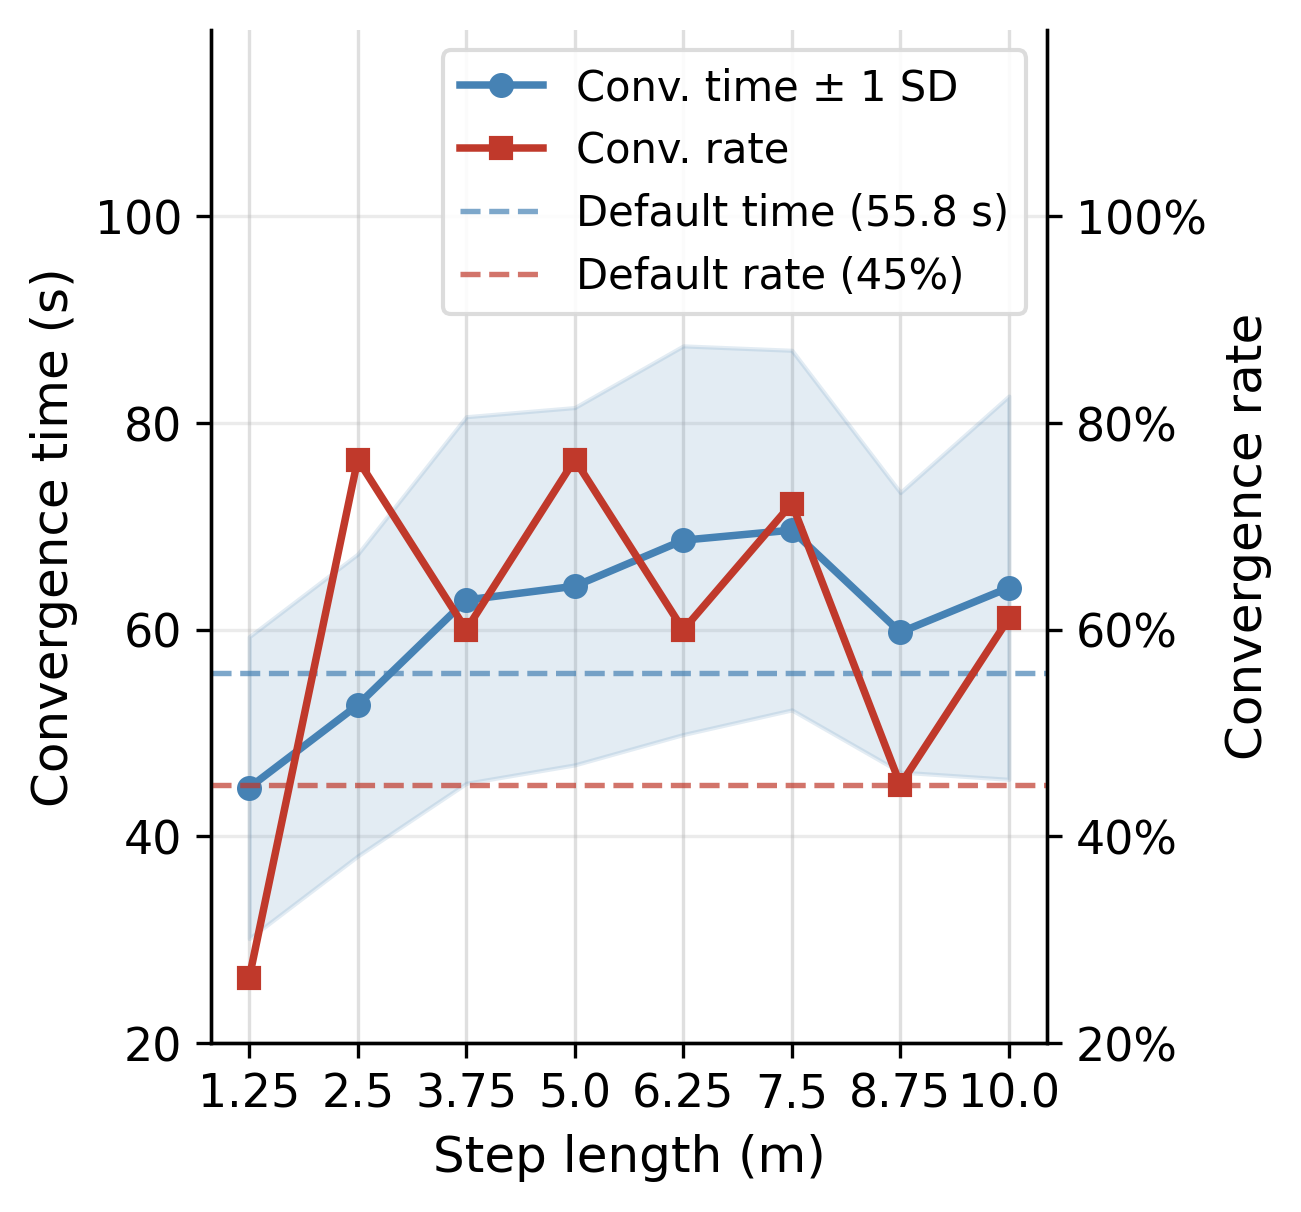
\includegraphics[width=\columnwidth]{img/experiments/step_sweep_plot.png}
    \caption{Convergence rate and mean convergence time ($\pm$1\,SD, converged runs only)
             as a function of fixed step length (20 seeds each).
             Steps of 2.5 and 5.0\,m yield the highest convergence rate (76\,\%).
             The rightmost group is the default configuration with adaptive step scaling
             enabled (base $d = 4$\,m), which achieves only 45\,\% convergence, worse
             than most fixed-step alternatives.}
    \label{fig:step_sweep}
\end{figure}

The shape of the response follows from how step length relates to the sensor range (5m).
Upon arriving at a candidate waypoint, the UAV has already sensed the forward direction
up to 5m ahead throughout its approach.
When new candidates are placed within that radius ($d < 5$m, e.g.\ $d = 1.25$m), the
area directly ahead is already pheromone-marked before any new candidate is ever generated
there.
The scoring function consequently never selects a forward-facing candidate, forcing the
agent into lateral or backward moves at every step.
This produces constant direction reversals rather than coherent coverage, and explains the
low 26\% convergence rate at $d = 1.25$m.
At the opposite extreme ($d \geq 8.75$m), candidates are placed so far from the UAV that
the pheromone values at those positions are entirely unrepresentative of the local coverage
state.
The scoring function no longer encodes a meaningful spatial gradient and directional choice
becomes effectively arbitrary.
The sweet spot at $d \in \{2.5, 5.0\}$m places candidates near the boundary of the sensed
area, where pheromone levels are fresh, locally informative, and varied enough to guide
consistent progress.
The adaptive mechanism underperforms for the same reason as long fixed steps.
Enlarging the ring in response to locally high pheromone density pushes candidates beyond
the sensed neighbourhood, reintroducing the uninformative signal before clusters are fully
confirmed.

\subsection{Full Factorial Sweep}

We evaluate the UAV-SAR model using a full factorial sweep over four key ACO parameters: candidate count, step length, pheromone exponent $\alpha$, and staleness exponent $\beta$. Candidate count is varied over $\{12,18,24,30,36\}$, step length over $\{50,75,100,125,150\}$, $\alpha$ over $\{0.5,1.0,1.5,2.0,2.5\}$, and $\beta$ over $\{1.0,1.5,2.0,2.5,3.0,3.5,4.0\}$. This yields 875 parameter combinations per seed.

We first validate the sweep with 3 seeds before scaling to the full run. The validation batch completed all expected runs (2,625/2,625 rows in \texttt{run\_summary.csv}) with a convergence rate of 95.85\% (2,516 converged, 109 timeouts). After validation, we execute the full 10-seed sweep for a total of 8,750 runs.

The full run also completed all expected parameter-seed combinations (8,750/8,750 rows). Overall convergence is 93.84\% (8,211 converged runs, 539 timeouts). At configuration granularity, 525 out of 875 parameter combinations achieved 100\% convergence across all 10 seeds, indicating a broad robust operating region.

Main effects show that step length is the strongest reliability lever: the shortest step ($d=50$) has the lowest mean convergence rate (0.822), while $d=100$ is highest (0.981). Candidate count is non-monotonic: moderate values ($n \in \{12,18,24\}$) outperform denser rings ($n \in \{30,36\}$). This pattern is consistent with a decentralized exploration-exploitation balance where overly dense local candidate sets can delay global closure.

The visual diagnostics in Figures~\ref{fig:fullfactorial_dashboard}--\ref{fig:fullfactorial_tradeoff} summarize the main structure of the sweep. The dashboard combines the step/candidate reliability map, the $\alpha$--$\beta$ interaction map, the reliability--time trade-off, and the seed-stability profile in a single compact overview. The top-15 bar chart then isolates the fastest fully-converged settings.

\begin{figure*}[ht]
  \centering
  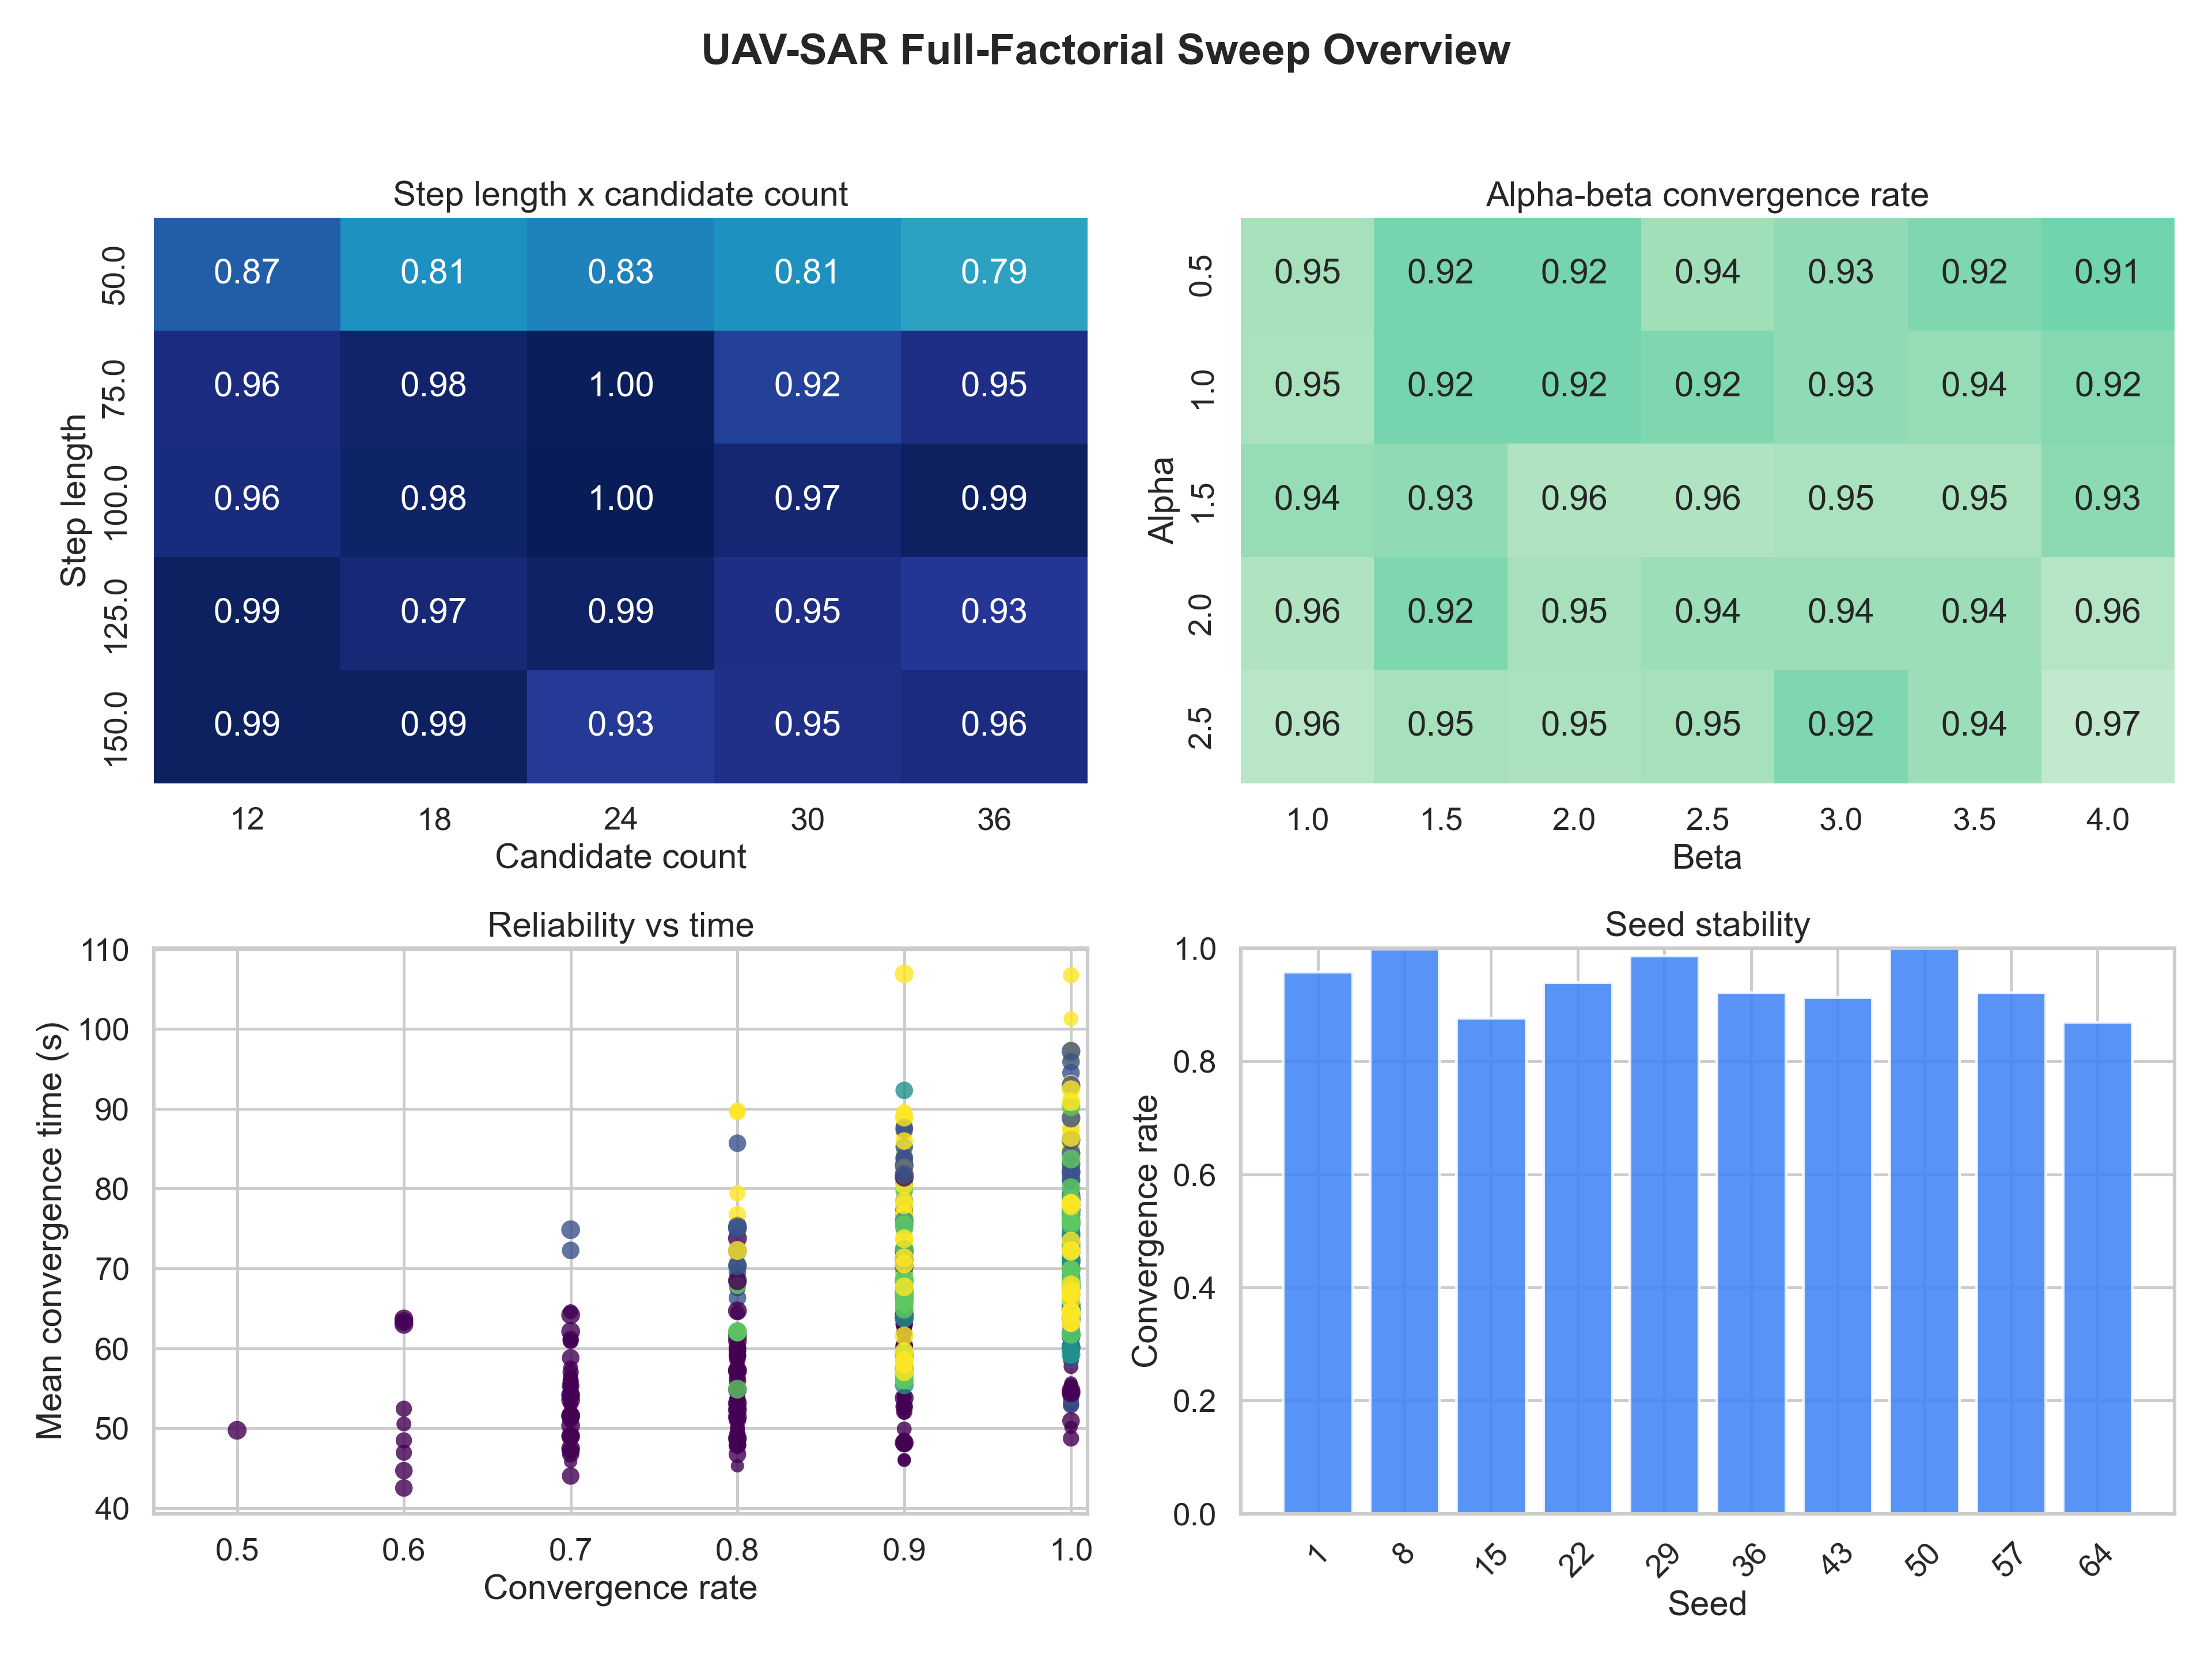
\includegraphics[width=0.92\textwidth]{img/experiments/full_factorial_20260601003651074/full_factorial_dashboard.png}
  \caption{Compact overview of the full-factorial sweep. The four panels summarize the dominant interaction surfaces, the reliability--time trade-off, and the seed-level stability pattern.}
  \label{fig:fullfactorial_dashboard}
\end{figure*}

\begin{figure*}[ht]
    \centering
    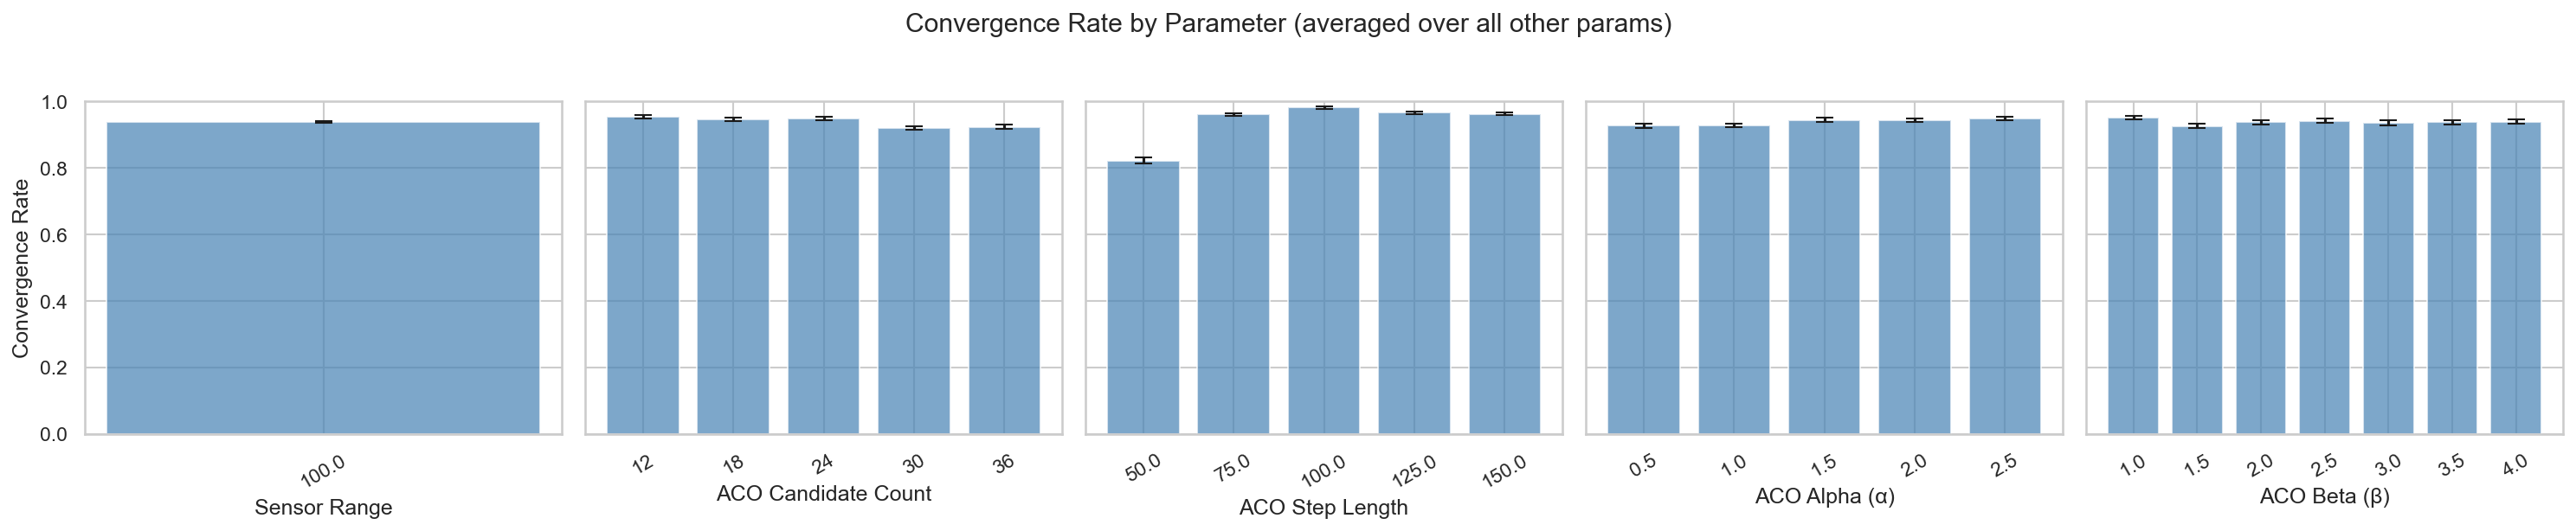
\includegraphics[width=0.49\textwidth]{img/experiments/full_factorial_20260601003651074/marginal_convergence_rate.png}
    \hfill
    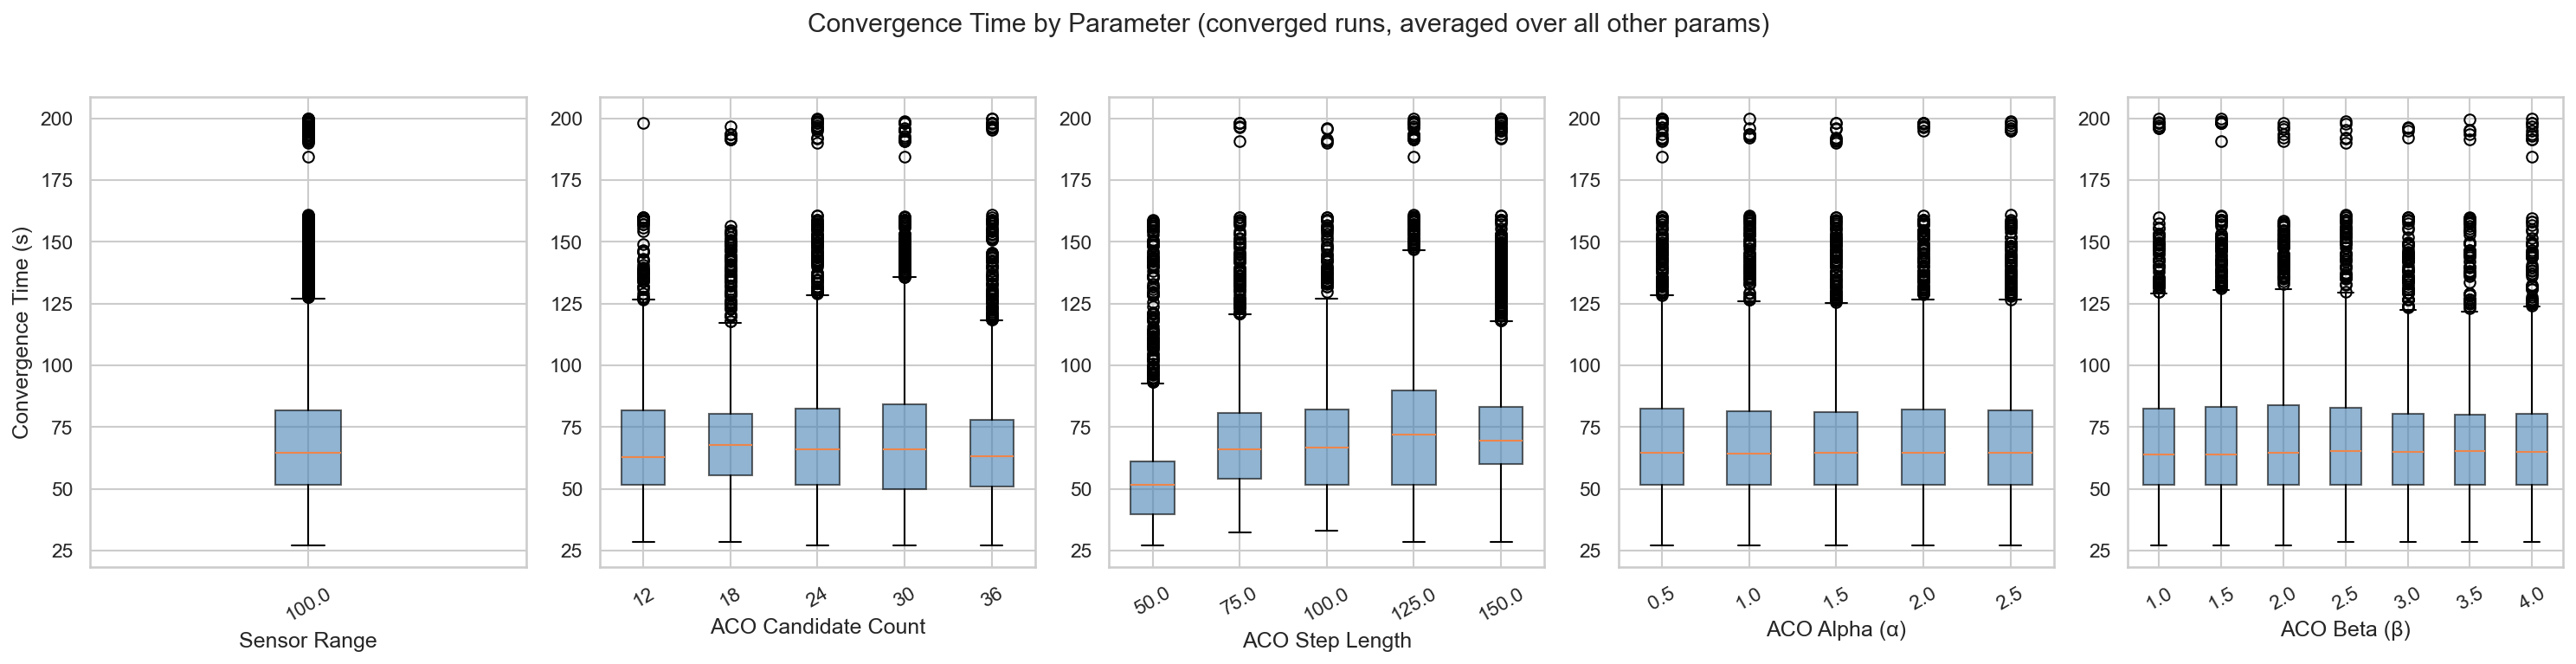
\includegraphics[width=0.49\textwidth]{img/experiments/full_factorial_20260601003651074/marginal_convergence_time.png}
    \caption{Full-factorial marginal effects (8,750 runs). Left: convergence-rate distributions by parameter value. Right: convergence-time distributions for converged runs. Reliability drops sharply at the shortest step length, while intermediate-to-long steps preserve high completion rates.}
    \label{fig:fullfactorial_marginals}
\end{figure*}

\begin{figure*}[ht]
    \centering
    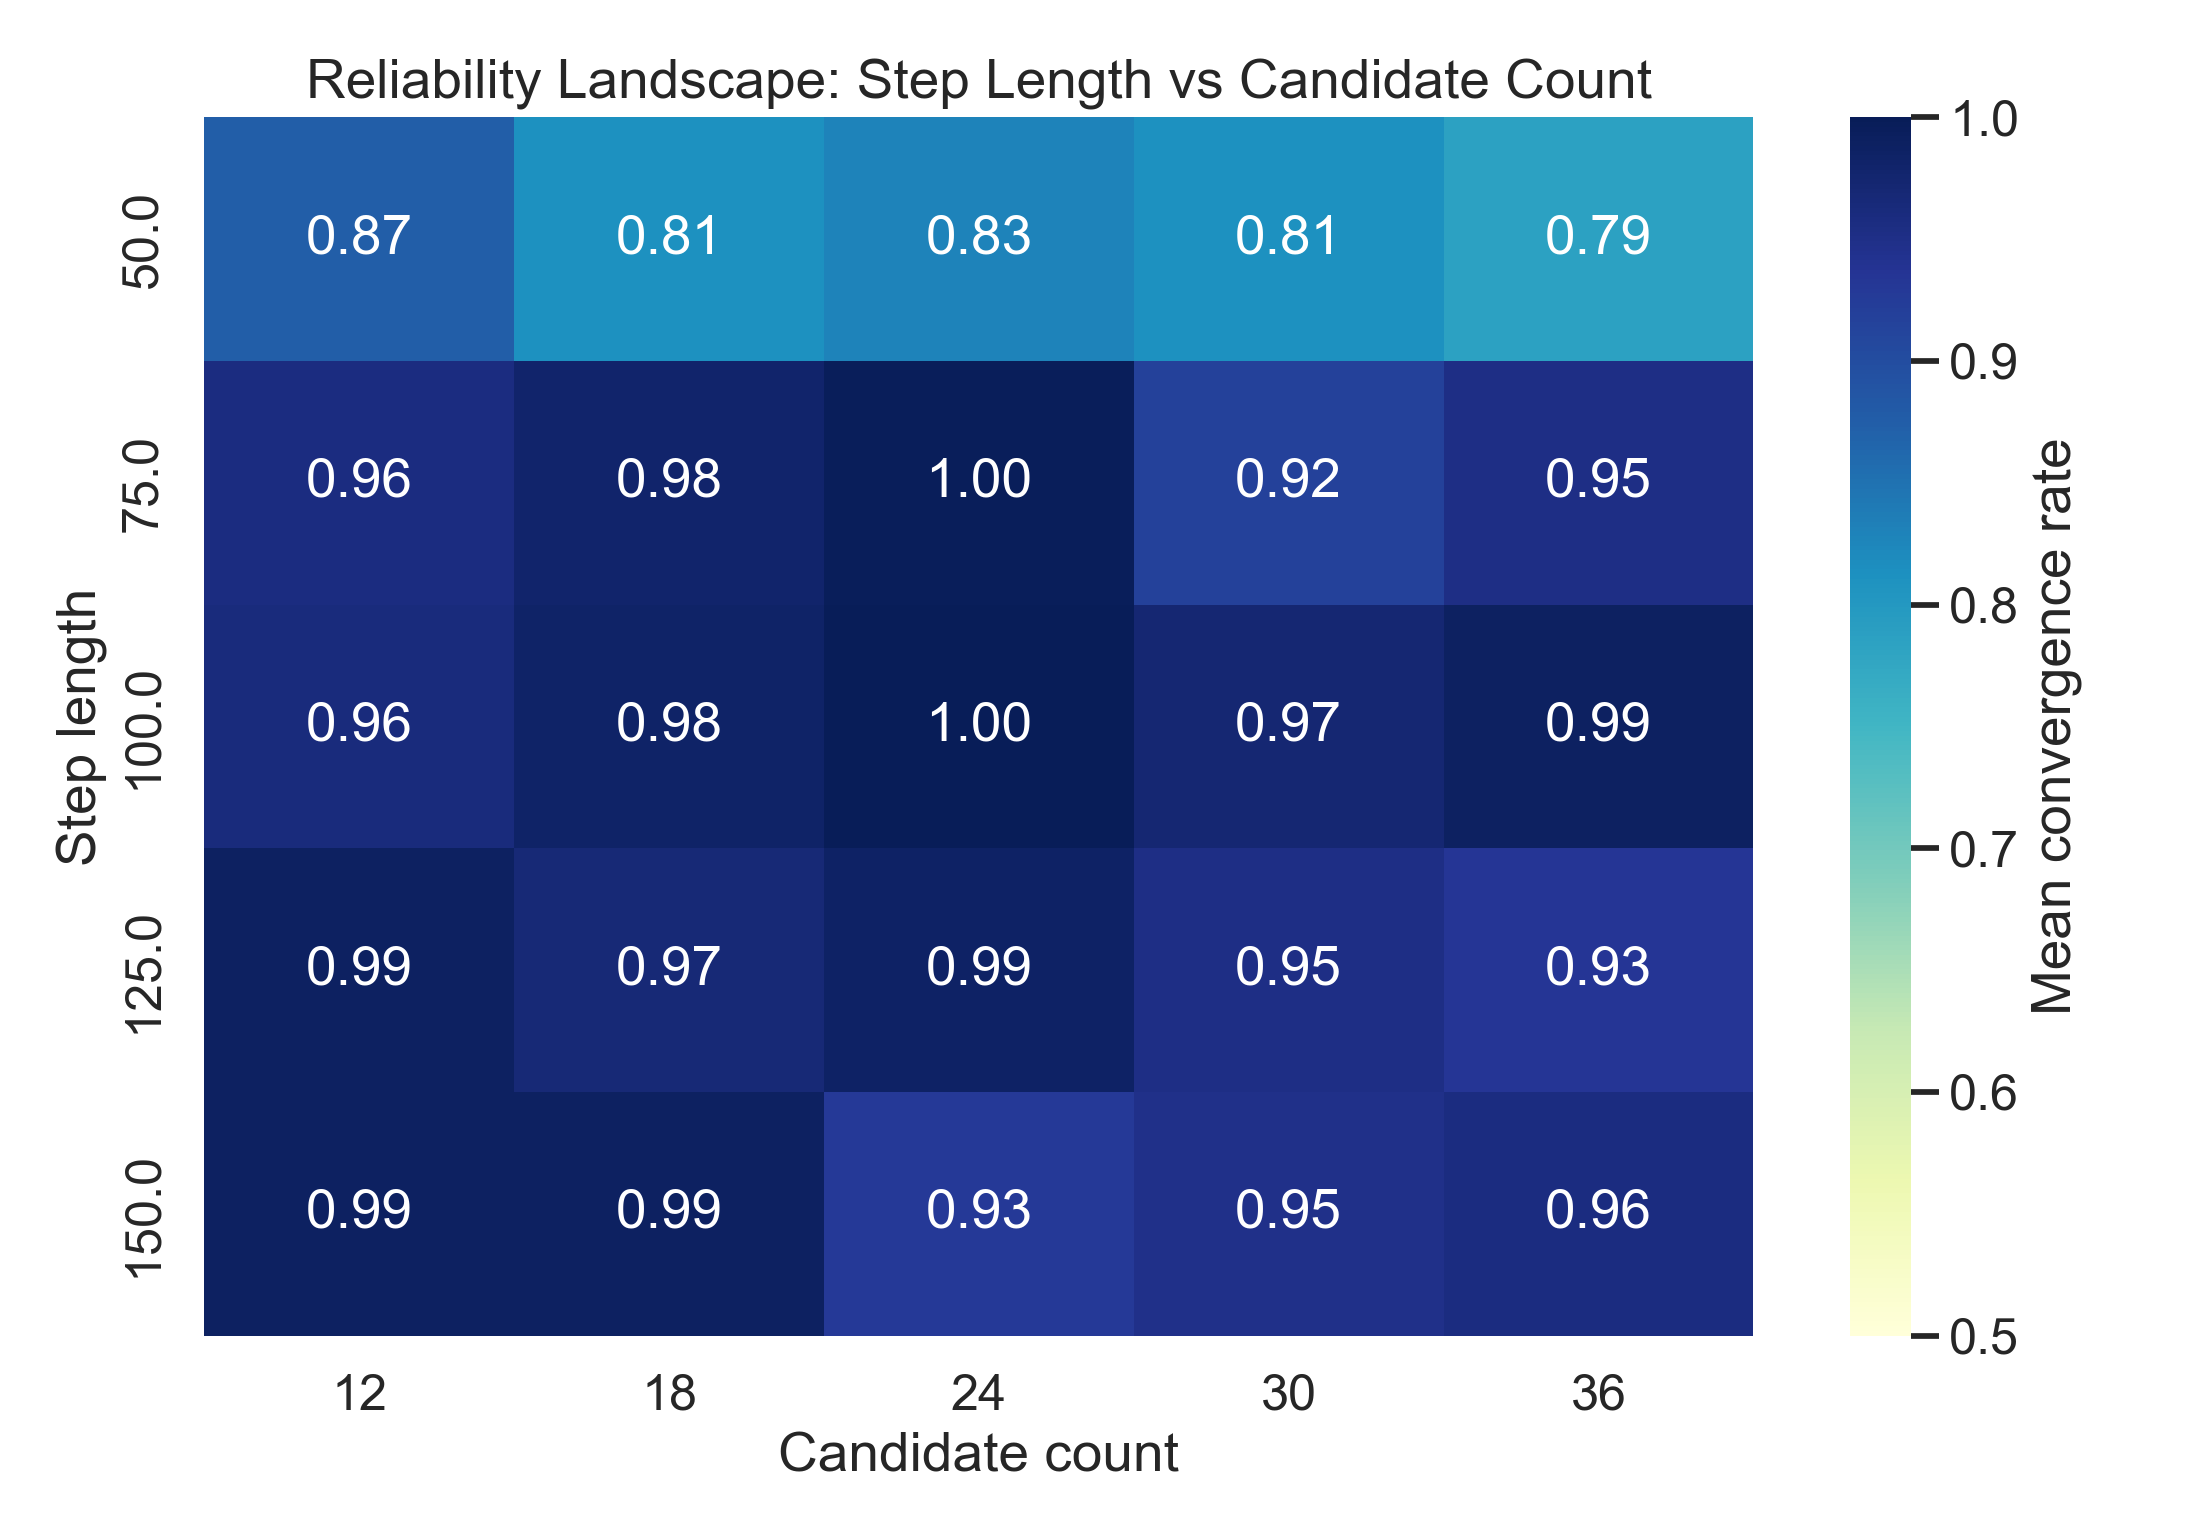
\includegraphics[width=0.49\textwidth]{img/experiments/full_factorial_20260601003651074/heatmap_step_candidate_rate.png}
    \hfill
    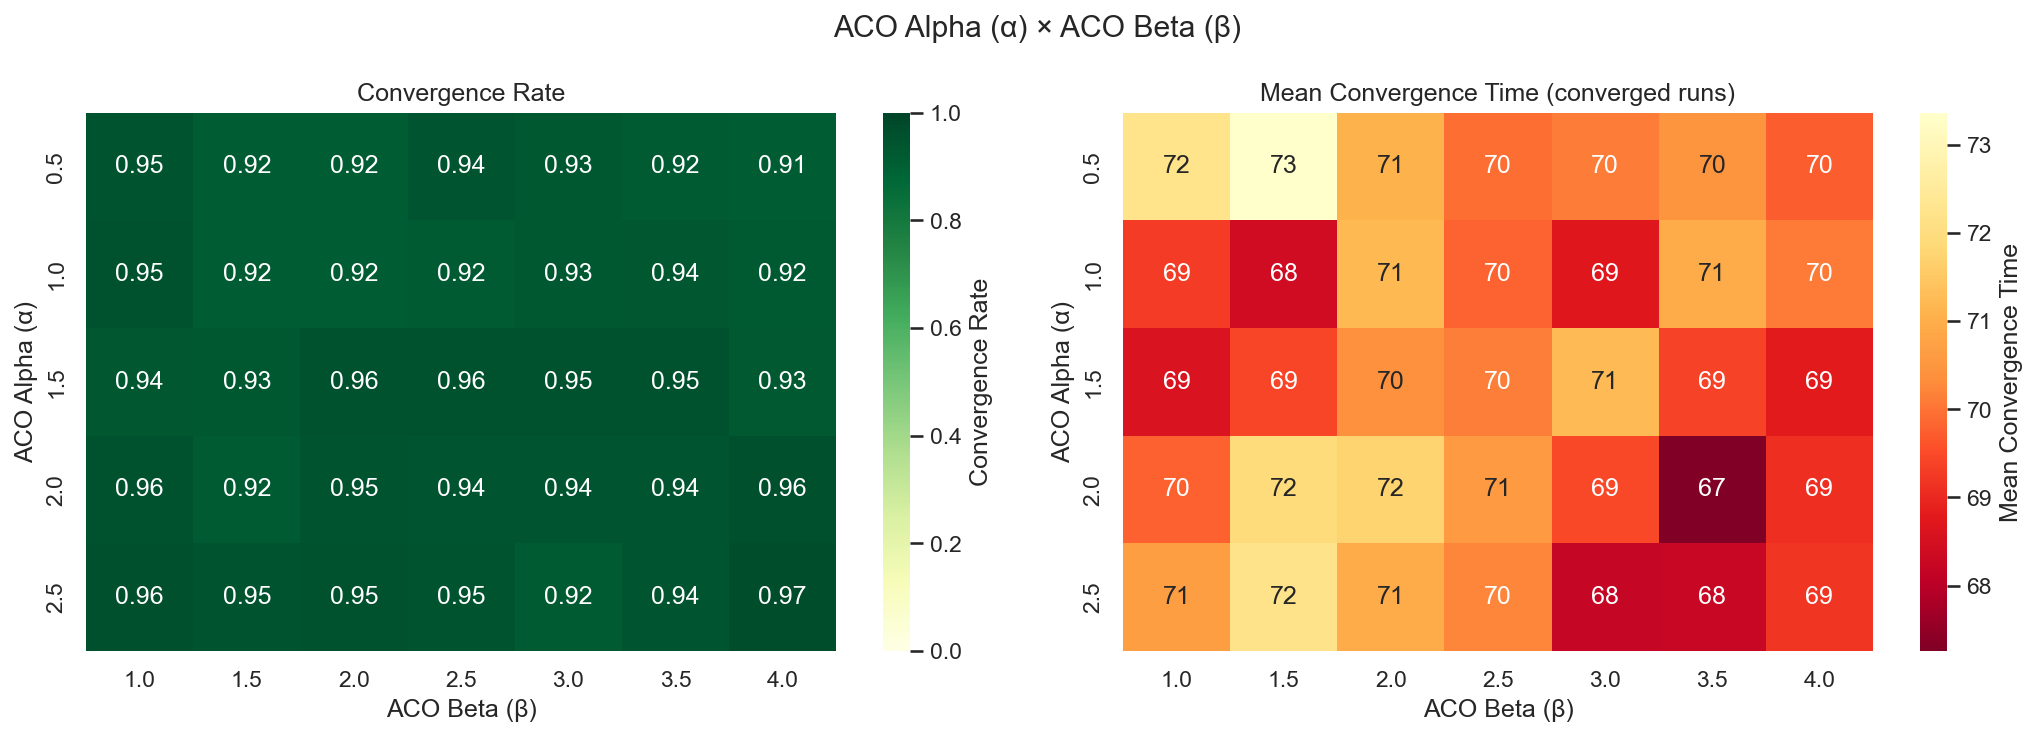
\includegraphics[width=0.49\textwidth]{img/experiments/full_factorial_20260601003651074/heatmap_alpha_beta.png}
    \caption{Full-factorial interaction views. Left: mean convergence rate over step length and candidate count. Right: reliability structure over $(\alpha,\beta)$. The dominant trough appears in short-step/high-candidate regions, while exponent effects are smoother and secondary.}
    \label{fig:fullfactorial_interactions}
\end{figure*}

\begin{figure*}[ht]
    \centering
    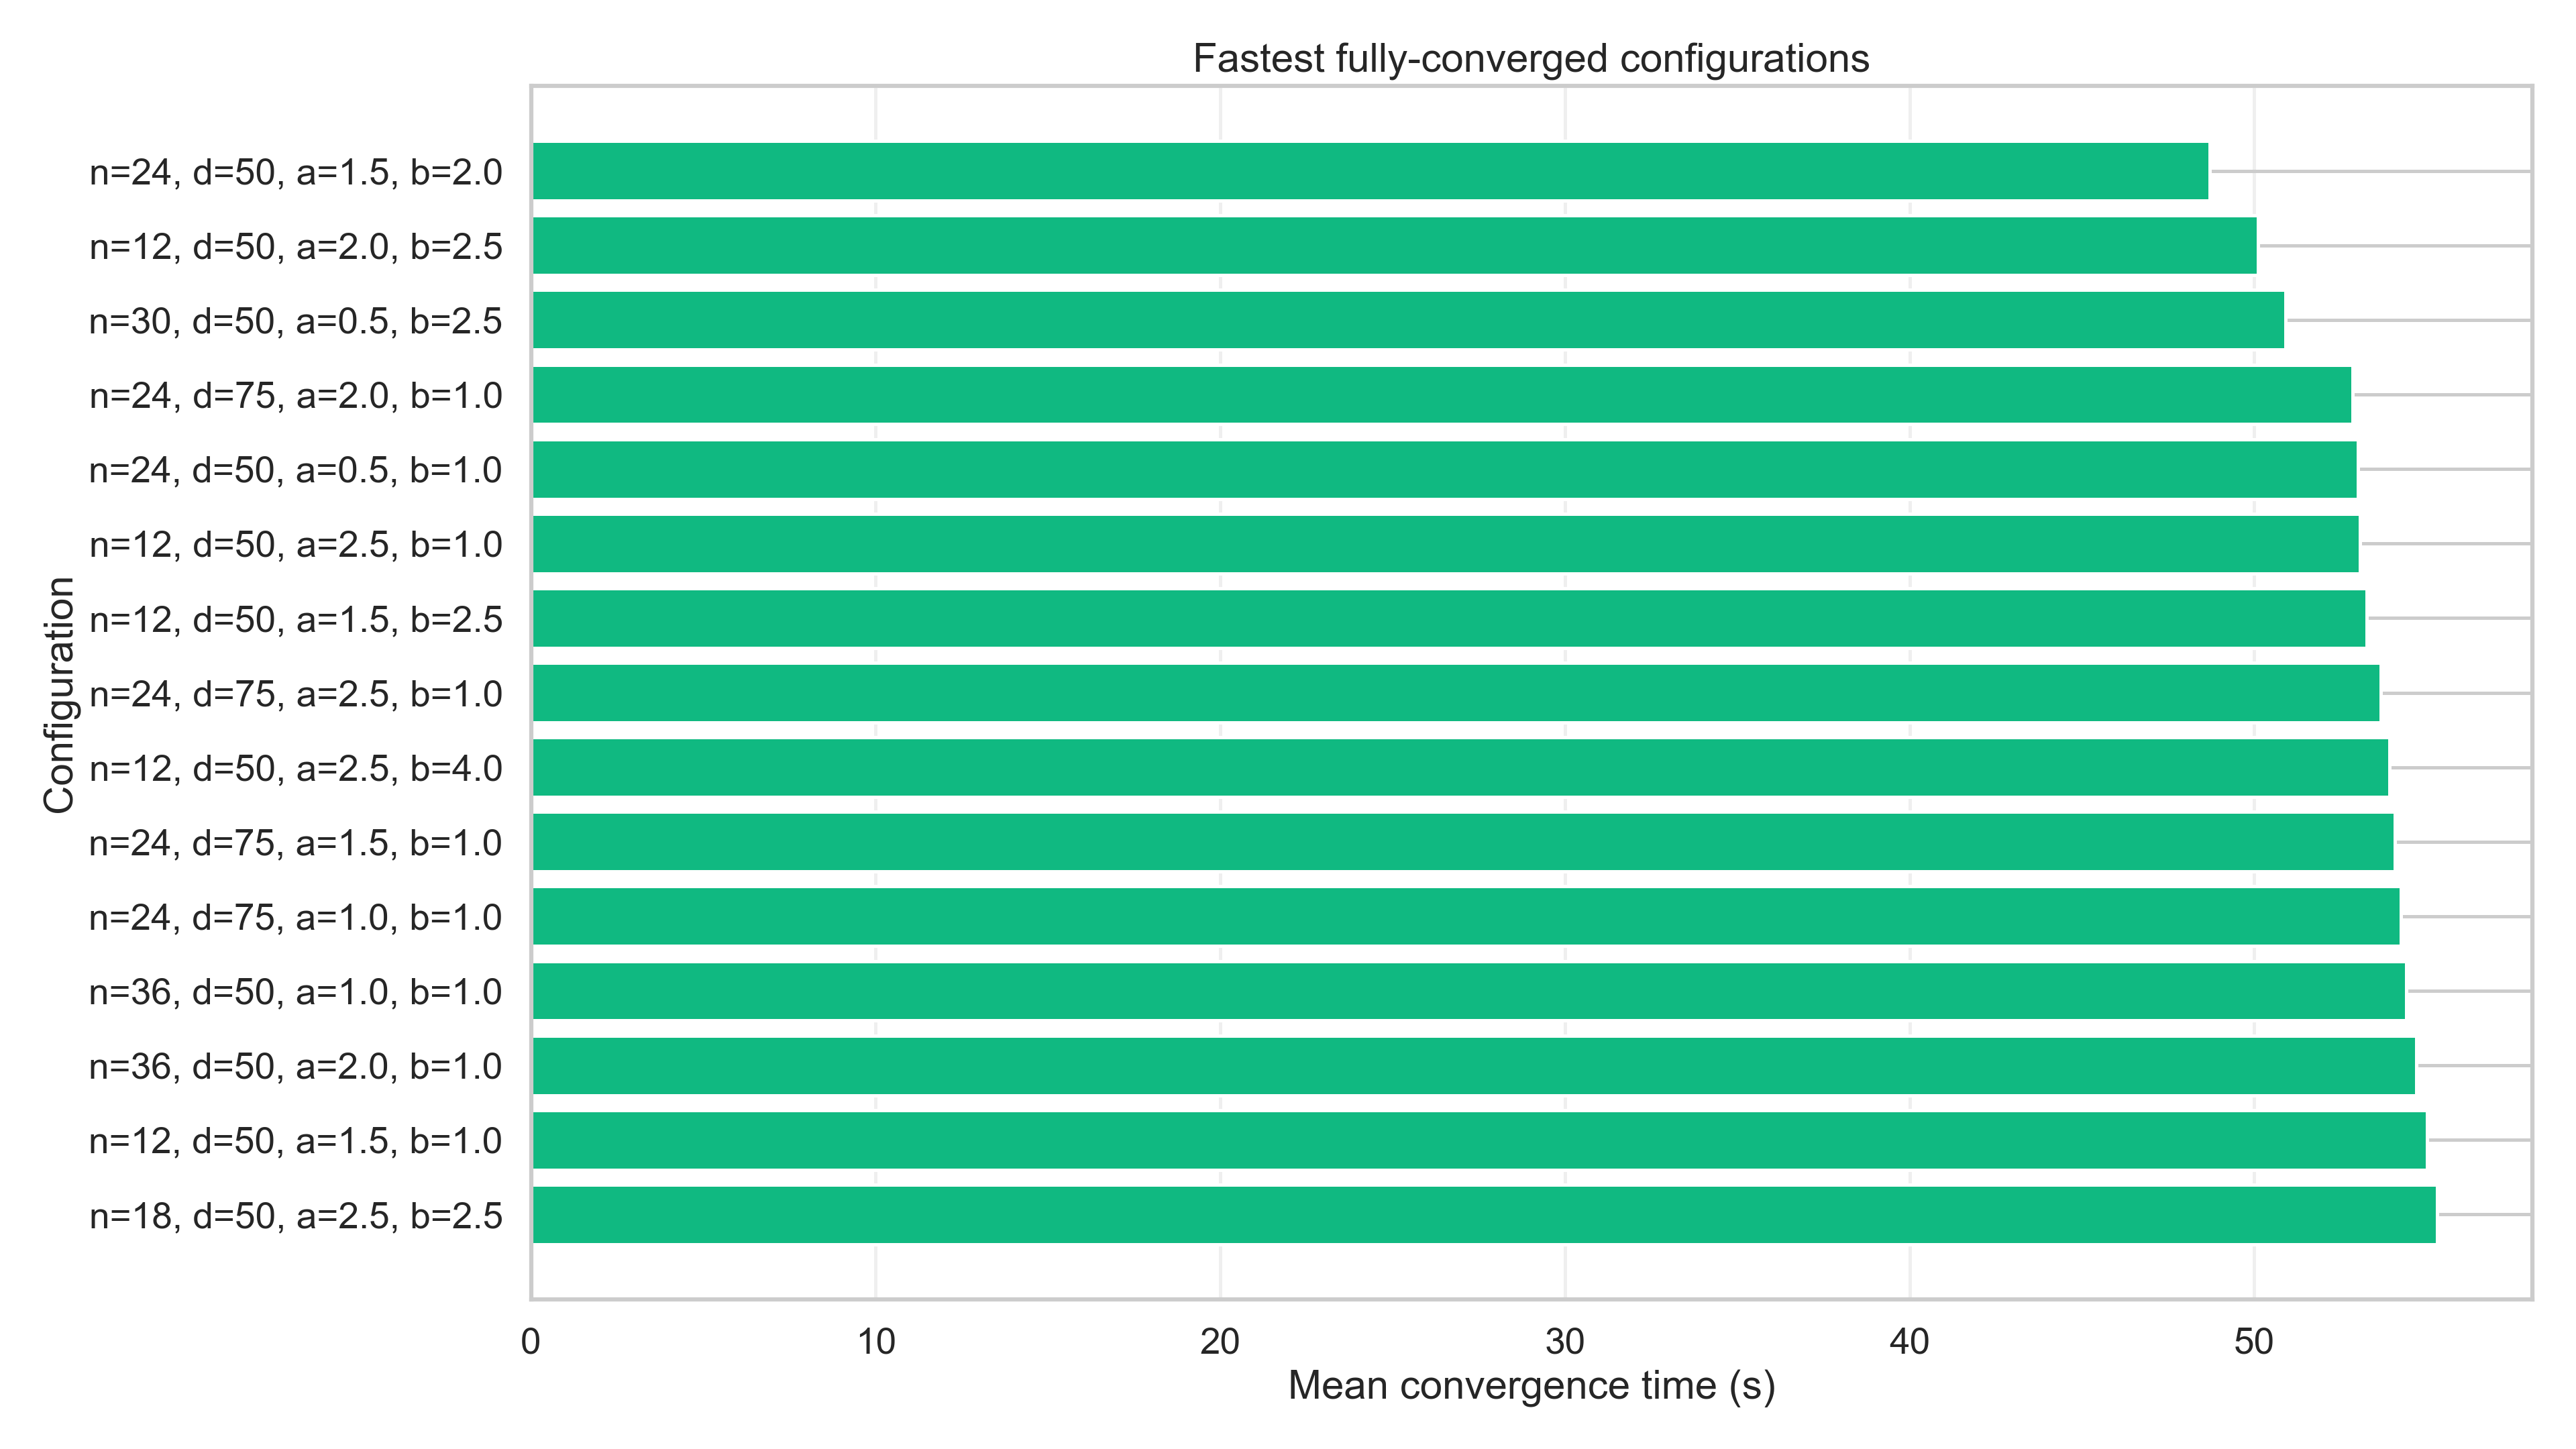
\includegraphics[width=0.49\textwidth]{img/experiments/full_factorial_20260601003651074/top15_full_converged.png}
    \hfill
    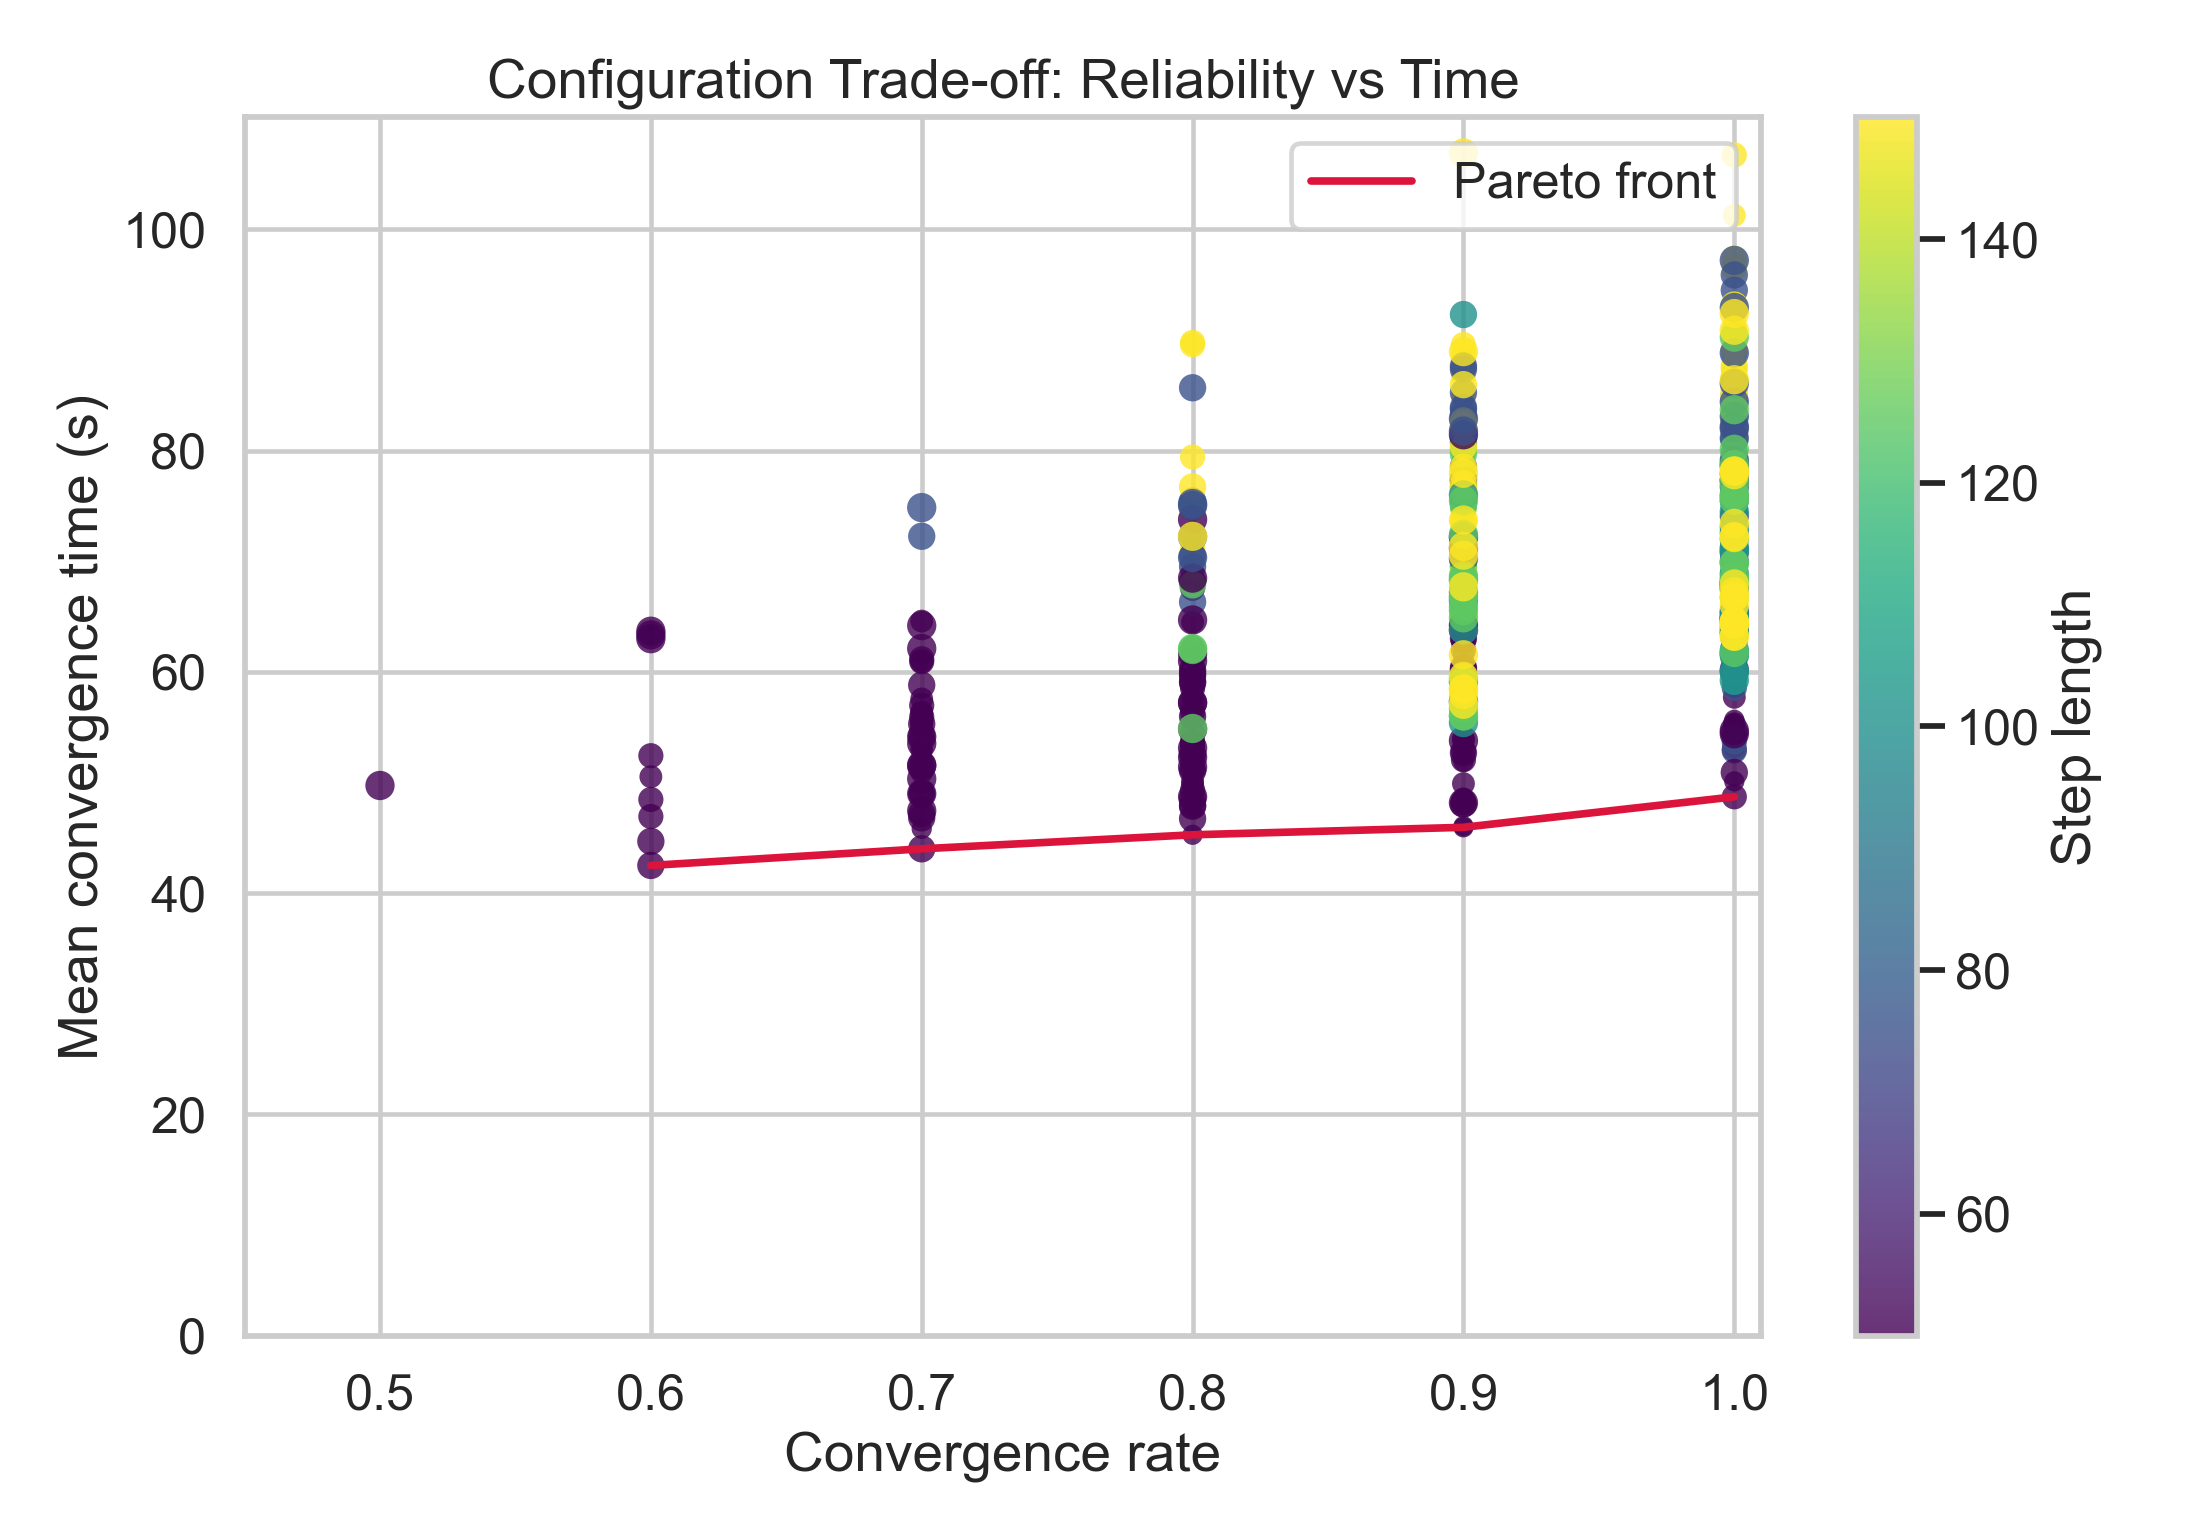
\includegraphics[width=0.49\textwidth]{img/experiments/full_factorial_20260601003651074/scatter_rate_vs_time.png}
    \caption{Summary diagnostics for the full-factorial sweep. Left: the fastest fully-converged configurations. Right: reliability--time trade-off across all 875 configurations with Pareto front overlay.}
    \label{fig:fullfactorial_tradeoff}
\end{figure*}

\subsection{Alpha--Beta Sensitivity}

A focused sweep over the ACO scoring exponents $(\alpha, \beta)$ in Equation~(2)
isolates how each term contributes to coverage performance. We vary both
exponents on the same grid $\{0.0, 0.5, 1.0, 1.5, 2.0, 2.5, 3.0\}$, deliberately
including the boundary at zero so the degenerate single-term scoring functions
appear as corner cases. This produces a $7 \times 7$ design of $49$ parameter
combinations. All other parameters are held at their defaults ($n = 24$,
$d = 4\,\text{m}$, sensor range $5\,\text{m}$), and each combination is
replicated over $21$ random seeds, giving $1029$ runs in total.

Convergence rate varies between $52\,\%$ and $76\,\%$ across the grid, and mean
convergence times among converged runs span $58$ to $71\,\text{s}$. The
dominant variation is along the $\beta$ axis. Columns with $\beta = 0$
consistently underperform, achieving only $52\text{--}57\,\%$ convergence;
once $\beta \geq 0.5$, convergence climbs into the $62\text{--}76\,\%$ band
and stays there. The $\alpha$ axis shows no comparable trend: at any fixed
$\beta \geq 1.0$, varying $\alpha$ from $0$ to $3$ shifts convergence rate by
at most $15$ percentage points and the response is non-monotonic. The worst
cell in the grid, $(\alpha, \beta) = (2.0, 0.0)$, achieves only $52\,\%$
convergence with a mean time of $70.6\,\text{s}$. The best convergence rates
($76\,\%$) appear at several cells, all with $\beta \geq 2.0$ and otherwise
unrelated $\alpha$ values, including $(0.0, 3.0)$, $(0.5, 2.0)$, and
$(2.5, 2.5)$. The fastest mean convergence times ($58\text{--}61\,\text{s}$)
cluster around moderate $\alpha$ and high $\beta$, with $(0.0, 3.0)$ and
$(0.0, 2.5)$ leading at roughly $61\,\text{s}$.

\begin{figure}[t]
  \centering
  
\includegraphics[width=0.95\columnwidth]{img/heatmap_alpha_beta.png}
  \caption{Convergence rate (left) and mean convergence time among
    converged runs (right) across the $7 \times 7$ grid of
    $(\alpha, \beta)$ values, $21$ seeds per cell. The $\beta = 0$
    column underperforms uniformly; $\alpha$ shows no comparable
    trend at fixed $\beta \geq 1$.}
  \label{fig:heatmap-ab}
\end{figure}

The asymmetry between $\alpha$ and $\beta$ follows directly from the scoring
function in our reversed-ACO formulation. Pheromone $\tau_i$ and freshness
$f_i$ are both updated inside the same \textsc{ExploreSense} tick: the same
sensor sweep that stamps a cell as freshly observed also deposits pheromone
on it. The two signals are therefore highly correlated, encoding the same
underlying fact (``this cell was visited recently'') in two different forms.
When $\beta > 0$, the staleness term $\eta_i^{\beta}$ already carries this
information, so further weighting the pheromone term through a larger $\alpha$
adds little independent directional signal. The $\beta = 0$ column is
qualitatively different because $\eta_i^{0} = 1$ collapses the staleness
contribution entirely, leaving the UAV with only the pheromone term, and
that signal alone is too coarse to consistently guide the swarm toward
unexplored ground.

This refines the broader observation made at the start of Section~6 that
$\beta$ has limited measurable effect. The effect is not absent: it has a
threshold structure. Moving from $\beta = 0$ to $\beta > 0$ measurably
improves convergence, but further increases past $\beta \approx 1$ provide
diminishing returns, consistent with our low-evaporation setup in which cells
never genuinely age out. No $(\alpha, \beta)$ cell achieved $100\,\%$
convergence across all $21$ seeds, indicating that the seed-to-seed variance
in GMM victim placement imposes a ceiling that local rule choices alone
cannot lift. For practical use, the default $(\alpha, \beta) = (1.0, 2.0)$
sits inside the high-convergence region of the grid, and the model is
largely insensitive to small departures from it.

% ─────────────────────────────────────────────────────────────────────────────
\section{Conclusion}
% ─────────────────────────────────────────────────────────────────────────────

We present a decentralized model of UAV-based search and rescue combining BDI-inspired statechart reasoning with a reversed ACO coordination mechanism. The design deliberately prioritizes interpretability alongside performance: every behavioral mode is a named state, every transition carries an explicit condition, and the coordination mechanism reduces to a single scoring formula. The statechart structure makes the system auditable in a way that a monolithic controller cannot offer. Each state handles exactly one responsibility and the overall organization reflects the MAS design principle of decentralized, structured agency. This makes the system easier to reason about, explain, and debug, even if it does not provide mechanical formula-level tracing from a single parameter change to a specific output difference.

The full-factorial sweep shows that the decentralized controller is not only interpretable but also calibratable. Step length is the strongest performance lever, candidate count introduces a non-monotonic trade-off, and the most fragile configurations cluster in the short-step, high-candidate regime. In contrast, a broad robust region remains stable across seeds and many parameter combinations converge consistently. These results show that local stigmergic rules generate predictable global reliability patterns without centralized coordination, which is precisely the type of emergent behavior this model was designed to expose.

\lipsum[7]

The model's simplifications define the boundaries of its validity. The environment is obstacle-free and two-dimensional. Real terrain constrains UAV trajectories in ways the model does not capture. The sensor is idealized, providing binary detection within a clean geometric cone with no noise, no false positives, and no occlusion. Coordination runs entirely through the shared pheromone grid, which presupposes a lossless shared data structure rather than an explicit radio channel. Victim positions are static. These simplifications are deliberate: they isolate the behavioral mechanisms of interest from confounding physical factors. But they establish the ceiling on the model's direct applicability.

Extending the model toward real-world deployment would require addressing each of these gaps. A probabilistic sensor model would replace the binary threshold with a Bayesian confidence update, accumulating evidence over multiple sensor passes and supporting partial detections. The shared pheromone grid would become a distributed gossip protocol. Each UAV would maintain a local copy and periodically merge it with neighbors within radio range, introducing communication latency and network partitions as new performance variables. Battery management would need hardware-specific discharge curves that account for wind, payload, and temperature. Regulatory constraints (altitude limits, beyond-visual-line-of-sight certification, and mandated collision avoidance margins) would impose hard trajectory constraints beneath the statechart layer.

Despite these gaps, the core design principles validated here transfer cleanly to more physically realistic architectures. Repulsive stigmergy for coverage dispersion, attractive stigmergy for exploitation, and a transparent statechart for inspectable behavioral switching are not artifacts of the simplified model. They are general principles applicable to any representation of recently-searched space, any detection model that produces a confidence signal, and any behavior architecture that supports explicit state modelling. The sensitivity analysis framework developed here provides a methodology that can be carried forward to guide calibration as the model is progressively extended toward deployment.


\balance
\bibliography{Bib.bib}

% \clearpage
% \appendix
% \onecolumn
% % ─────────────────────────────────────────────────────────────────────────────
\section{Experimental Details}
% ─────────────────────────────────────────────────────────────────────────────

All distances are in metres.

\paragraph{Environment and Main agent.}
Table~\ref{tab:params_main} lists the fixed environment and victim-placement parameters.

\begin{table}[h]
\centering
\caption{Environment and Main agent parameters.}
\label{tab:params_main}
\begin{tabular}{lll}
\toprule
Parameter & Value & Notes \\
\midrule
Search area            & 45\,$\times$\,25\,m         & \\
UAV count              & 2                           & \\
Victim count           & 5                           & \\
Pheromone grid         & 90\,$\times$\,50 cells      & 0.5\,m/cell \\
Evaporation rate $\rho$& 0.01\,s$^{-1}$              & Lazy exponential decay \\
GMM clusters           & 2                           & \\
GMM weights            & \{0.2,\;0.5\}               & Normalised \\
GMM std dev (cluster 1)& 3.5\,$\times$\,3.5\,m       & \\
GMM std dev (cluster 2)& 1.5\,$\times$\,1.5\,m       & \\
GMM boundary margin    & 1.5\,m                      & \\
Safety timeout         & 100\,s                      & \texttt{varMaxSimTime} \\
\bottomrule
\end{tabular}
\end{table}

\paragraph{UAV agent.}
Table~\ref{tab:params_uav} lists the UAV-level parameters. Parameters marked
\emph{swept} are varied in the experiments; all others are fixed at the values shown.

\begin{table}[h]
\centering
\caption{UAV agent parameters (defaults). Swept parameters are varied in experiments.}
\label{tab:params_uav}
\begin{tabular}{lll}
\toprule
Parameter & Value & Notes \\
\midrule
Speed                         & 0.05\,m/s                 & \\
Sensor range                  & 5.0\,m                    & \\
FOV half-angle                & 45$^\circ$                & \\
Detection threshold           & 0.7                       & \\
Pheromone deposition rate     & 2.0 per cell              & \\
Staleness constant $T_\text{stale}$ & 60\,s             & \\
Candidate count $n$           & 24                        & \emph{swept} \\
Step length $d$               & 4.0\,m                    & \emph{swept} \\
ACO exponent $\alpha$         & 1.0                       & \emph{swept} \\
ACO exponent $\beta$          & 2.0                       & \emph{swept} \\
UAV avoidance radius          & 9.0\,m                    & Score penalty zone \\
Min UAV separation            & 10.0\,m                   & Hard avoidance \\
Adaptive step enabled         & false                     & Disabled in step sweep \\
Adaptive step threshold       & 1.0 (pheromone)           & Triggers scale-up \\
Adaptive step max multiplier  & 2.0                       & Maximum $M$ \\
Local search radius           & 8.75\,m                   & Post-confirmation bias \\
Battery initial level         & 100\,\%                   & \\
Battery depletion rate        & 0.5\,\%/s                 & Effective in-flight rate \\
Battery return threshold      & 20\,\%                    & Triggers move-to-charger \\
Charging rate                 & 10\,\%/s                  & At charging station \\
Charger location              & (44,\;23)\,m              & Bottom-right corner \\
\bottomrule
\end{tabular}
\end{table}


\end{document}
